%! Author = moeve
%! Date = 22.01.2025

\documentclass[12pt, norsk]{article}

% Pakker
\usepackage{amsfonts}
\usepackage{amsmath}
\usepackage{amssymb}
\usepackage{amsthm}
\usepackage{babel}
\usepackage{caption}
\usepackage{colortbl}
\usepackage{csquotes}
\usepackage{fancyhdr}
\usepackage{gauss}
\usepackage{geometry}
\usepackage{graphicx}
\usepackage{hyperref}
\usepackage{listings}
\usepackage{mathtools}
\usepackage{multicol}
\usepackage{multirow}
\usepackage{nicefrac}
\usepackage{pdfpages}
\usepackage{physics}
\usepackage{ragged2e}
\usepackage{scalerel}
\usepackage{subcaption}
\usepackage{times}
\usepackage{url}
\usepackage{wasysym}
\usepackage{wrapfig}
\usepackage{xcolor}


% Margstørrelser. Gitt av Diego
\geometry{left=25mm, bottom=25mm, 
right=25mm, top=25mm}

% Store romertall som sidetall de første sidene
\pagenumbering{Roman}

% Sidetallene skal være nedre høyre
\pagestyle{fancy}
\renewcommand{\headrulewidth}{0pt}   % Ingen linje på toppen
\fancyhead{}   % "Frigjør" headerne
\fancyfoot{}
\fancyfoot[R]{\thepage}

% Inputter forskjellige ting som trengs
\usepackage[style=apa, 
            language=norsk,
            backend=biber]{biblatex}
            \DefineBibliographyStrings{norsk}{%
  andothers = {et\addabbrvspace al\adddot}
}
\addbibresource{bibliografi.bib}
\usepackage{csquotes}
\newcommand{\doubleSignature}[5]{
\begin{tabular}{lll}
\rule{5.5cm}{1pt} & \phantom{\rule{5.5cm}{1pt}}&  \\
#1, #2 & & \\ 
& & \\ 
& & \\ 
& & \\ 
    \rule{4cm}{1pt} & \rule{4cm}{1pt} & \rule{4cm}{1pt} \\
    #3 & #4 & #5
\end{tabular}
\vspace{1cm}
}
\lstset{literate=%
{æ}{{\ae}}1
{ø}{{\o}}1
{å}{{\aa}}1
{Æ}{{\AE}}1
{Ø}{{\O}}1
{Å}{{\AA}}1
}

\definecolor{codegreen}{rgb}{0,0.6,0}
\definecolor{codegray}{rgb}{0.5,0.5,0.5}
\definecolor{codepurple}{rgb}{0.58,0,0.82}
\definecolor{backcolour}{rgb}{0.9,0.98,1}

\lstdefinestyle{mystyle}{
    backgroundcolor=\color{backcolour},   
    commentstyle=\color{codegreen},
    keywordstyle=\color{magenta},
    numberstyle=\tiny\color{codegray},
    stringstyle=\color{codepurple},
    basicstyle=\ttfamily\normalsize,
    breakatwhitespace=false,  
    numbers=left,
    breaklines=true,                 
    captionpos=b,                    
    keepspaces=true,                            numbersep=8pt,                  
    showspaces=false,                
    showstringspaces=false,
    showtabs=false,                  
    tabsize=2
}
\lstset{literate=%
{æ}{{\ae}}1
{ø}{{\o}}1
{å}{{\aa}}1
{Æ}{{\AE}}1
{Ø}{{\O}}1
{Å}{{\AA}}1, style=mystyle
}




% Dokumentet
\begin{document}

% Forsiden. Må prøve å gjøre mere latexvennlig. enn så lenge PDF fra Word
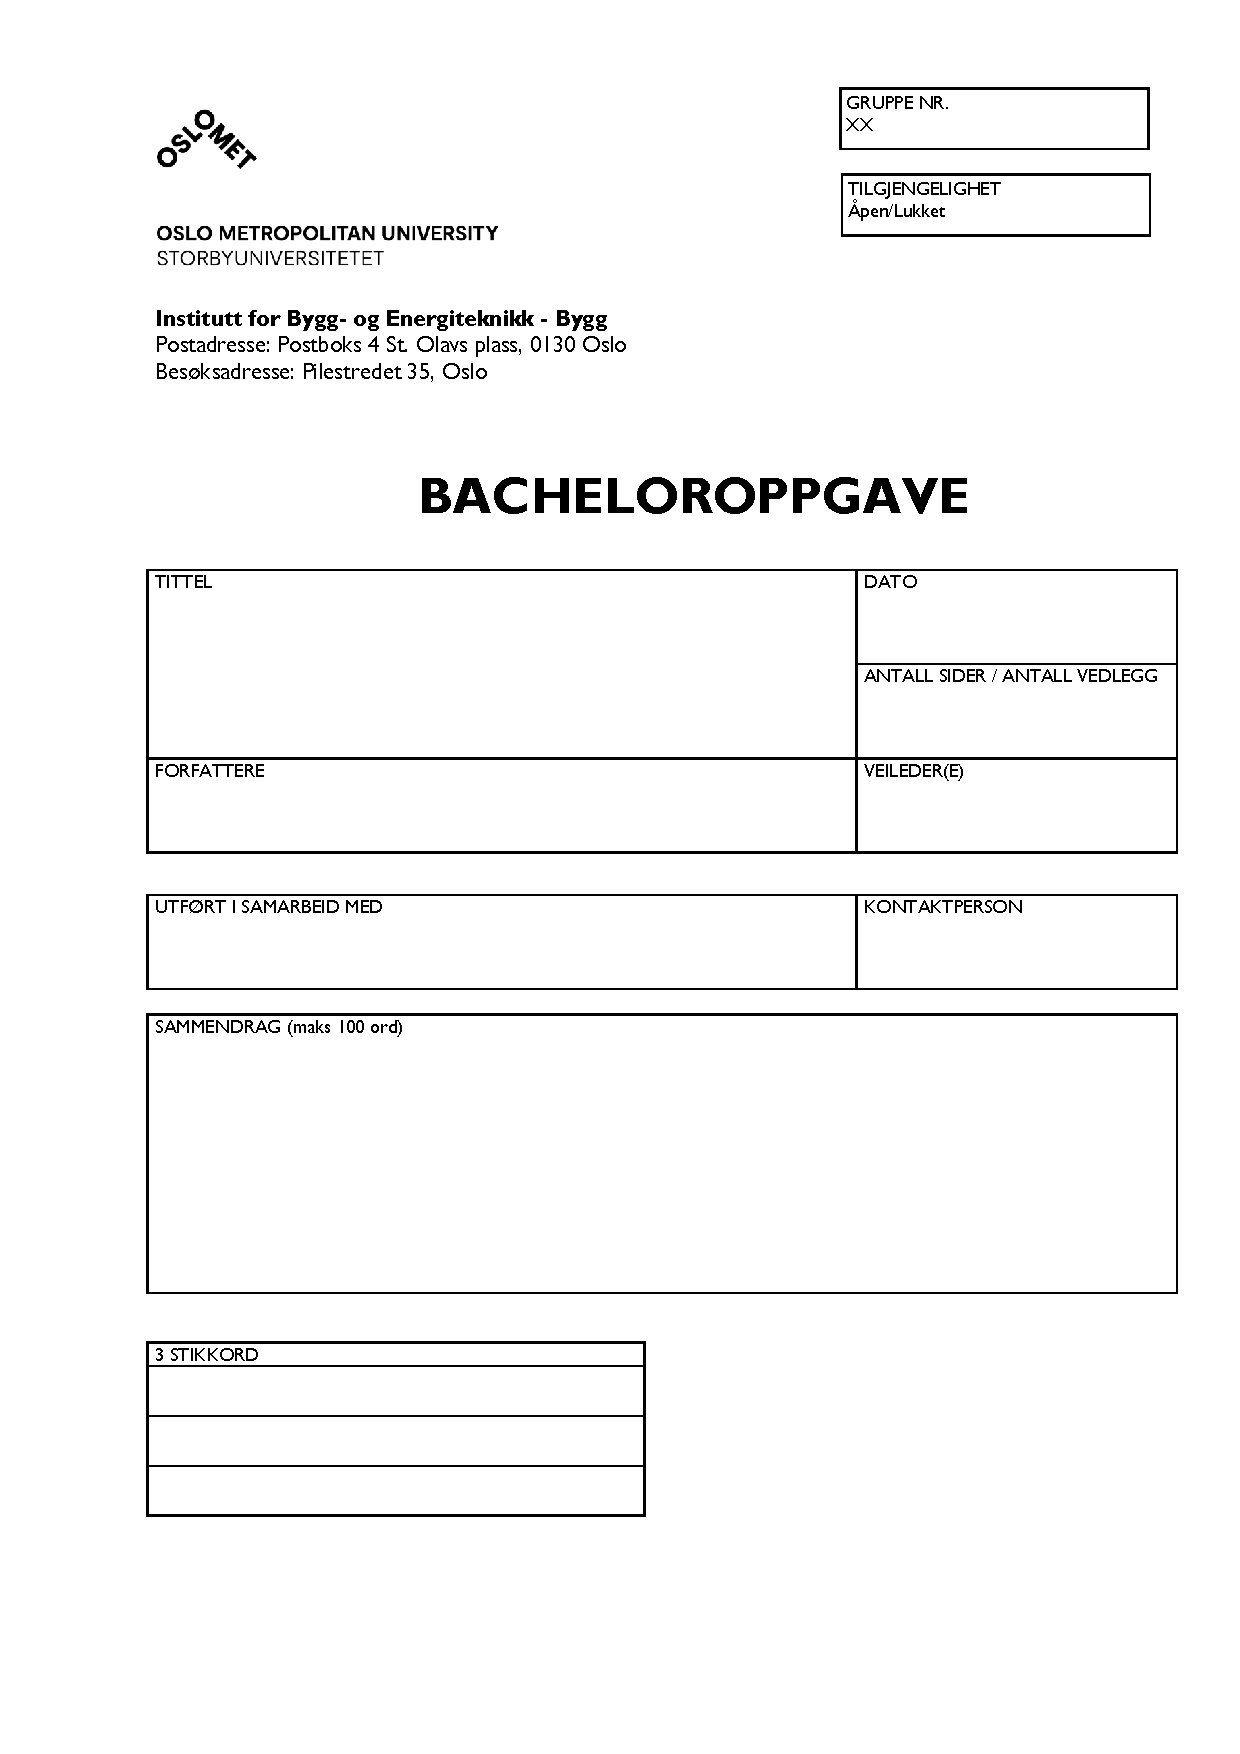
\includepdf[pages=-]{3 PDFS/BSc-oppgave.pdf}

% Forord
\section*{FORORD}




\vfill 
\doubleSignature{Oslo}{\today}{Antonio Kaelin}{Espen Karlsen}{Martin Øvergård}



\newpage

% Sammendrag
\section*{SAMMENDRAG}
\newpage

% Abstract
\section*{ABSTRACT}
\section*{Innholdsfortegnelse..}
\section*{Liste over forkortelser, symboler, figurer og tabeller evt.}
\newpage

% Hoveddel. Arabiske tall
\pagenumbering{arabic}
\setcounter{page}{1}

% Innledning
\section{INNLEDNING}


\subsection{Bakgrunn}
\subsection{Avgrensninger}
\newpage

% Teori
\section{Teori}

\subsection{Modalanalyse (omega, modeshape, måling med mobil/frequency, FFT)} 
\subsection{ANN (weights, bias, architechture, training/testing/validation, activation layers, regularization etc)}
\newpage

% Metode
\input{F METODE/Metode}
\subsection{SOFiSTiK-analyse i Python}
\subsection{ANN-kode (parametre brukt/prøvd? antall batches? antall layers? antall neurons? hva slags act. functions? etc.}
\newpage

% Case study
\section{Case study}
\newpage

% Resultater
\section{Resultater}
\newpage

% Diskusjon
\section{Diskusjon}
\newpage

% Konklusjon
\section{Konklusjon}

% Bibliofi APA 7
\printbibliography
\newpage

% Vedlegg. Små romanske tall
\pagenumbering{roman}
\setcounter{page}{1}
\appendix

% Vedleggene
\section{Vedlegg 1}

% Ferdig
\end{document}
